%% LyX 2.0.6 created this file.  For more info, see http://www.lyx.org/.
%% Do not edit unless you really know what you are doing.
\documentclass{llncs}

\usepackage[utf8]{inputenc}
\usepackage[english]{babel}
\usepackage{amssymb}
\usepackage{algorithm}
\usepackage{algorithmicx}
\usepackage[noend]{algpseudocode}


%\usepackage{amsthm}
%\theoremstyle{definition}

\newcommand*\Let[2]{\State #1 $\gets$ #2}
\algrenewcommand\algorithmicrequire{\textbf{Input:}}
\algrenewcommand\algorithmicensure{\textbf{Output:}}
\algrenewcommand\algorithmicrequire{\textbf{Input:}}
\algrenewcommand\algorithmicensure{\textbf{Output:}}
\newcommand{\ti}{\textit}

%\usepackage{tablefootnote}
\begin{document}

\title{Interaction Components Between Components based on a Middleware}

\author{Van Cam Pham, Ansgar Radermacher}

\institute{CEA, LIST, Laboratory of Model driven engineering for embedded systems,\\Point Courrier 174, Gif-sur-Yvette, F-91191 France\\
\email{name.surname@cea.fr}
}



\maketitle

\begin{abstract}
The so-called model-driven engineering approach relies on two paradigms, abstraction and automation, recognized as very efficient for dealing with complexity of today system. 
%Abstraction is the ability to provide simplified and focused view of a system and requires adequate modeling language. 
%For this concern, it is clear that the Unified Modeling Language (UML) is nowadays the most used, educated, documented and tooled modeling language. 
%Even, if a graphical language such as the UML is not the silver bullet for all software related concerns, it provides hence better support than text-based solutions for some concerns such as architecture and logical behavior of application development. 
UML state machine and their visual representations are much more suitable to describe logical behaviors of system entities than any equivalent text based description such as IF-THEN-ELSE or SWITH-CASE constructions. Although many industrial tools and research prototypes can generate executable code from such graphical language, their support only focus special cases of UML state machine, especially non-concurrent state machines. While UML state machine concepts such as concurrency, pseudo states such as history, fork, junction and time events are widely used by software architects, the code generation of the existing approaches does not take these concepts into account. To blur the boundaries between the modeling and coding worlds, a code generator should be able to generate code from all concepts of modeling languages with respect to the semantics described by the language specifications.

To this end, this paper proposes an approach to generate code from all UML state machines with all of its concepts with respect to the Precise Semantics of UML, especially concurrent state machines which are based on multi-thread-based design.
%After code modifications, round-trip engineering is needed to make the model and code consistent, which is a critical aspect to meet quality and performance constraint required from project manager today. Unfortunately, current UML tools only support structural concepts for round-trip engineering such as those available from class diagrams. In this paper, we address the round-trip engineering of UML state-machine and its related generated code. We propose a round-trip engineering approach consisting of a forward process which generates code by using transformation patterns, and a backward process which is based on code pattern detection to update the original state machine model from the modified generated code. We implemented a prototype and conducted several experiments on different aspects of the round-trip engineering to verify the proposed approach.
%\lipsum[1]
\end{abstract}

\section{\uppercase{Introduction}}
\label{sec:intro}
%1. Say the complexity, CPS .. UML SM is ...
%2. MDE ..., OMG defines powerful specification for USM..
%3. To blur the boundaries between... => need to have code generation
%4. Problem: 1. most of existing... focus only on sequency aspect..., many pseudo states are not supported while these pseudo states are widely used as powerful means to describe the dynamic behavior of system. 2. Concurrency is not taken into account. 3. Generated code is dependent on library of generation tools => not portable. Speed + executable size + runtime execution memory consumptio (for IoT)n + semantic conformance.
%To.... => this paper address the analysis for multithread-based concurrency code genration and the code generation for full UML state machine with respect to the specification...
%Contribution: Concurrency, systematic approach for code generation, evaluation conforming to UML precise semantics...
%Structure

%Internet of Things \cite{Li2015} drives the complexity of embedded systems today rapidly increases. 
%Today embedded systems directly interacting with running environment does not run in standalone mode but also react to the system environment changes. 
%Event-driven architecture \cite{Michelson2006} is an useful way to design such systems, in which events come to the system either from outside (data) or inside the system itself (time event or internal changes). 
The UML State Machine (USM) \cite{Specification2007} and its visualizations are efficient to model the behavior of event-driven architecture.   
%USM defines how systems behave in case of changes. 
%The rise in use of the Model-Driven Engineering (MDE) approach promotes the automation in software development. 
Tools and approaches are proposed to automatically translate USMs into executable code in the context of Model-Driven Engineering (MDE) \cite{Mussbacher2014}.%, which are recognized as very efficient for dealing with system complexity. 
%Automation is to reduce the gap between the modeling world
%, which consists of software architects, who prefer using graphical languages such as USM, 
%and the implementation world
%, which involves programmers 
%by bringing the ability to automatically generating code from diagram-based modeling languages such as USM to executable code.  
%The gap between the modeling world, which consists of software architects, who prefer using graphical languages such as USM, and the implementation world, which involves programmers, is therefore reduced. 

However, despite many advantages of MDE and USM, they are not widely adopted as a recent survey revealed \cite{1030}.
This is partially due to poor support for code generation \cite{forward2010perceptions}.

On one hand, the usefulness and semantics of USM are being empowered by OMG by providing more concepts and their precise semantics such as pseudo states and composite state machines. 
On the other hand, existing code generation tools and approaches have some issues regarding completeness, semantics and efficiency of generated code. 
Existing approaches either support a subset of USM modeling concepts or handle composite state machines by flattening into simple ones with a combinatorial explosion of states, and excessive generated code \cite{badreddin2014enhanced}.
%is language-dependent and still limited to simple cases, especially when considering concurrency of \ti{doActivity} and orthogonal regions, pseudo states such as history, and different events. 
%This again enlarges the gap between the USM semantics and the actual generated code.
Specifically, the following lists some of the current issues: 
\vskip 0.1cm
\noindent
\tb{Completeness:} Existing tools and approaches mainly focus on the sequential aspect while the concurrency of state machines is limitedly supported. 
Pseudo states are not rigorously supported by existing tools such as Rhapsody 
	%does not support \ti{doActivity}, junctions, and truly concurrent execution of orthogonal regions
	\cite{ibmdiff}.
	%Concurrency of is often implemented sequentially. 
	%Sinelabore \cite{sinelabore} does not support fork, join, junction and concurrent states. 
	%Rhapsody and Enterprise Architect \cite{EA} only support \ti{CallEvent} and \ti{TimeEvent} while \ti{SignalEvent} and \ti{ChangeEvent} are missing. 
	%Pseudo states such as history, choice and junction are poor \cite{EA,sinelabore} while these are very helpful in modeling.
Designers are then restricted to a subset of USM concepts during design.

\vskip 0.1cm
\noindent	
\tb{Efficiency:} Code generated from tools such as Rhapsody \cite{ibm_rhapsody} and FXU \cite{Pilitowski2007} depends on the libraries provided by the tool vendor, which makes the generated code non portable. 
Event processing speed and executable file size of generated code are not optimized \cite{6195875}.
	
\vskip 0.1cm
\noindent
\tb{Semantics:} The semantics of UML State Machine is defined by a recent OMG-standardized: Precise Semantics of State Machine (PSSM) \cite{OMG2015}.
This standard is not (yet) taken into account for validating the runtime execution semantics of generated code. 

%In order for wider integrating MDE into software development today, one task is to seamlessly make the behavior of the code generated from UML State Machine complied with the semantics specified by PSSM. 
Given the above issues, the objective of this paper is to present a novel code generation pattern and its tooling support. 
The latter offers efficient code generated from USMs with full concepts to reduce the modeling-implementation gap.   

The proposed pattern extends IF-ELSE constructions with our support for concurrency. 
%The tool also supports \ti{deep separation} for separating USM-prescribed code and user action code,
Runtime execution of generated code is experimented with the PSSM test suite.
%Although supporting multi-thread-based concurrency, binary files compiled from and the event processing speed of runtime execution of code generated by our approach are dramatically smaller than some manual implementation approaches and code generation tools.
  
%Abstraction provides simplified and focused views of a system and requires adequate graphical modeling languages such as Uni. Even, if the latter is not the silver bullet for all software related concerns, it provides better support than text-based solutions for some concerns such as architecture and logical behavior of application development. UML state machines (USMs) and their visual representations are much more suitable to describe logical behaviors of system entities than any equivalent text based descriptions. The gap from USMs to system implementation is reduced by the ability of automatically generating code from USMs  \cite{Booch1998, Douglass1999,Shalyto2006,Douglass1999}. 

%Ideally, a full model-centric approach is preferred by MDE community due to its advantages \cite{Selic2012}. However, in industrial practice, there is significant reticence \cite{Hutchinson:2011:MEP:1985793.1985882} to adopt it.
%On one hand, programmers prefer to
%use the more familiar textual programming language. 
%On the other hand, software architects, working at higher levels
%of abstraction, tend to favor the use of models, and therefore
%prefer graphical languages for describing the architecture of
%the system.
%However, on the one hand, maintaining code generated from existing approaches is non-trivial. On the other hand our observation is that it is very difficult to come up with formalizations that yield such elegant code generation solutions \cite{6032552}. In other words, generated code must be manually modified to build fully operational applications. 
%On one hand there are traditional developers who prefer to implement the system by writing code, while on the other hand there are developers who prefer to use entirely models for the design and implementation of the system. 
%The code modified by programmers and the model are then inconsistent. Round-trip engineering (RTE) \cite{Hettel2008} is proposed to synchronize different software artifacts, model and code in this case \cite{Sendall}. RTE enables actors (software architect and programmers) to freely move between different representations \cite{Sendall} and stay efficient with their favorite working environment. 

%After code modifications, round-trip engineering (RTE) is needed to make the model and code consistent, which is a critical aspect to meet quality and performance constraint required from project managers today. 
%Unfortunately, current industrial tools such as for instance Enterprise Architect \cite{sparxsystems_enterprise_2014} and IBM Rhapsody\cite{ibm_rhapsody} only support structural concepts for RTE such as those available from class diagrams and code. Compared to RTE of class diagrams and code, RTE of USMs and code is non-trivial. It requires a semantical analysis of the source code, code pattern detection and mapping patterns into USM elements. 
%This is a hard task, since mainstream programming languages such as C++ and JAVA do not have a trivial mapping between USM elements and source code statements.

%For software development, one may wonder whether this RTE is doable. That is, why do the industrial tools not support the propagation of source code modifications back to original state machines? Several possible reasons to this lack are (1) the gap between USMs and code, (2) not every source code modification can be reverse engineered back to the original model, and (3) the penalty of using transformation patterns facilitating the reverse engineering that may not be the most efficient (e.g. a slightly larger memory overhead). 
%in the mind of these tools' vendors, users always make changes to models rather than to code. Generated code, in these tools, is therefore not supposed to be changed directly.  

%In this paper, we address the RTE of UML State Machine diagrams and its related generated code. We propose a RTE approach consisting of a forward process which generates code by using transformation patterns, and a backward process which is based on code pattern detection to update the original state machine model from the modified generated code. From the proposed approach, we implemented a prototype and conducted several experiments on different aspects of the round-trip engineering to verify the proposed approach. 



%Model-driven engineering (MDE) is a development methodology aiming to increase software productivity and quality by allowing different stakeholders to contribute to the system description \cite{Mussbacher2014}. MDE considers models as first-class artifacts and generates code from higher abstraction level models. Recent survey \cite{1030} has revealed that industries are gaining the adoption of code generation into software development life-cycle. Although many tools and research prototypes can generate executable code from models, generated code could be manually modified by programmers, e.g. skeleton code generated from UML \cite{Specification2007} class diagrams. Models and the generated code are therefore out of synchronization. Round-trip engineering \cite{Aßmann200333, Hettel2008, E-ESE-120044648} (RTE) is proposed to keep the artifacts synchronized.

%RTE supports synchronizing different software artifacts, model and code in this case, and thus enabling actors (software architect and programmers) to freely move between different representations \cite{Sendall}. Tools such as for instance Enterprise Architect \cite{sparxsystems_enterprise_2014}, Visual Paradigm \cite{visual}, and AndroMDA \cite{_andromda_} provide RTE but most of them are only applicable for system structure models such as class diagrams.  

%This study addresses the RTE of UML State Machine (SM) and object-oriented programming languages such as C++ and JAVA. SM is widely used in practice for modeling the behavior of complex systems, notably reactive, real-time embedded systems. There are several approaches to generating source code from state machines or state charts such as nested switch/if statements \cite{Booch1998}, state-event-table \cite{Douglass1999, Duby2001}, and state pattern \cite{Allegrini2002,Shalyto2006,Douglass1999}. Unfortunately, the generated code from these approaches is very difficult for programmers to maintain without an appropriate supporting tool. RTE is impossible in these approaches even with very small changes such as changing transition targets or actions made to code. The reason behind this impossibility is that, in mainstream programming languages such as C++, JAVA, (1) there are not equivalents between SMs and source code statements and (2) the code generation pattern of these approaches has not been chosen with RTE in mind.

%This paper addresses the RTE of UML state-machines and object-oriented programming languages such as C++ and JAVA. The forward  engineering of the approach takes as input a state-machine and executes two transformations. The first is UML to UML by utilizing several transformation patterns such as the double-dispatch approach presented in \cite{spinke_object-oriented_2013} and the second is a generation of code from the transformed UML. Traceability information is stored, during the transformations. In the backward direction, a verification is executed by the code pattern detection to verify the correctness of the code before the backward process taking as input the modified generated code, the UML classes, the original state-machine and mapping information together merges changes from code to the state-machine. We implemented a prototype supporting RTE of state-machine and C++ code, and conducted several experiments on different aspects of the RTE to verify the proposed approach. To the best of our knowledge, our implementation is the first tool supporting RTE of SM and code. 
%The prototype also improves the collaboration between MDE developers and traditional programmers in developing reactive complex embedded systems.

%This paper addresses the RTE of USMs and object-oriented programming languages such as C++ and JAVA. The main idea is to utilize transformation patterns from USMs to source code that aggregates code segments associated with a USM element into source code methods/classes rather than scatters these segments in different places. Therefore, the reverse direction of the RTE can easily statically analyze the generated code by using code pattern detection and maps the code segments back to USM elements. Specifically, in the forward direction, we extend the double dispatch pattern presented in \cite{spinke_object-oriented_2013}. Traceability information is stored during the transformations. We implemented a prototype supporting RTE of state-machine and C++ code, and conducted several experiments on different aspects of the RTE to verify the proposed approach. To1 the best of our knowledge, our implementation is the first tool supporting RTE of SM and code. 

To sum up, the contributions of this paper are: (1) an approach and tooling support for code generation from USMs with full features; 
(2) an empirical study on the semantic-conformance and efficiency of generated code;
and (3) application of the tool to a case study.  

We assume that readers of this paper have knowledge about UML State Machine and its basic execution semantics.

The remaining of this paper is organized as follows: Section \ref{sec:modeling} describes the modeling of applications using UML State Machines. 
Section \ref{sec:uniqueness} mentions the features of our tool.
Thread-based concurrency is designed in Section \ref{sec:thread}. 
Based on this design, a code generation approach is proposed in Section \ref{sec:codegen}. 
The implementation and empirical evaluation are reported in Section \ref{sec:exp}. 
The application of our tool to a case study is presented in Section \ref{sec:casestudy}.
Section \ref{sec:relatedwork} discusses related work. The conclusion and future work are presented in Section \ref{sec:conclusion}.

\section{Background definition}
\label{subsec:background}

\begin{definition}A directed graph $G = \{V, Ed\}$ consists of a finite set $V$ of vertexes, and a set $Ed$ of edges. An edge connects a source vertex to a target vertex. The source and target vertexes of an edge ed are obtained by $src(ed)$ and $tgt(ed)$.
\end{definition}

\begin{definition}A UML vertex $v \in V$ has a kind $v.kind \in$  \ti{\{initial, final, state, comp, conc, join, fork, choice, junction, enpoint, expoint, history\}}. Each vertex $v$ has a name and we write $v.name$. 
\end{definition} 

\begin{definition}A region $r \in \mathcal{R}$ is composed of one or several vertexes, and contained by a state $s$. We write $ctner(r) = s$ and $subvts(r)$ is its sub-vertices set. 
\end{definition}	

\begin{definition} A UML state s is a vertex v where v.kind $\in$ {state, comp, conc}. s has an $entry$, an $exit$ and a $doActivity$ action. A composite state $cs$ contains one or more vertexes. We write $subvts(cs)$ is a set of vertexes contained by cs and $ctner(v)$ refers to the containing state of the vertex v. A concurrent state contains more than one region.
\end{definition}		

\begin{definition} An action $act$ $\in$ $ActLang$ is a set of statements written in an object-oriented programming language $ActLang$. A guard is a boolean expression written in $ActLang$.
\end{definition}

\begin{definition} A transition $t \in T$ is an edge connecting two vertexes. A transition has a guard $guard(t)$, an effect $effect(t)$, and is associated with a set of events $\subset$ E. We write $events(t)$ as the associated set of events. A transition has a type $t.type$ $\in \{trigger, triggerless, guardless\}$ and a kind $t.kind \in {external, local, internal}$.
\end{definition}

\begin{definition} An event is one of the followings:
	\begin{itemize}
		\item A \ti{TimeEvent} $te$ specifies the time of occurrence $d$ relative to a starting time. The latter is specified when a state, which accepts the time event, is entered.
		
		\item A \ti{SignalEvent} $se$ is associated with a signal $sig$, whose data are described by its attributes and is occurred if $sig$ is received by a component, which is an active UML class.
		
		\item A \ti{ChangeEvent} $che$ is associated with a boolean expression $ex(che)$ written in $ActLang$. $che$ is emitted if $ex(che)$ changes from true (false) to false (true).
		
		\item A \ti{CallEvent} $ce$ is associated with an operation $op(ce)$. $ce$ is emitted if there is a call to $op(ce)$.
	\end{itemize}
\end{definition}

\begin{comment}
\begin{definition} A \ti{TimeEvent} $te$ an internal event and specifies the time of occurrence $d$ relative to a starting time. The latter is specified when a state, which accepts the time event, is entered. 
\end{definition}

\begin{definition} A \ti{Signal} $sig$ is data described by its attributes. 
\end{definition}

\begin{definition} A \ti{SignalEvent} $se$ is associated with a signal $sig$ and is occurred if $sig$ is received by a component, which is an active UML class. 
\end{definition}	

\begin{definition}
	A \ti{ChangeEvent} $che$ is associated with a boolean expression $ex(che)$ written in $ActLang$. $che$ is emitted if $ex(che)$ changes from true (false) to false (true).
\end{definition}

\begin{definition}
	A \ti{CallEvent} $ce$ is associated with an operation $op(ce)$. $ce$ is emitted if there is a call to $op(ce)$.
\end{definition}
\end{comment}

Suppose that for each vertex \ti{v} $\in$ $V$, its incoming and outgoing transition lists are extracted by the functions $incomings$ and $outgoings$, respectively. For a list $l$, the function $head$ is used to get the first element of the list. If $v.kind = conc$, suppose $regions(v)$ is the region set contained by $v$. Given a transition t:
\begin{itemize}
	\item $t.type = trig$ if $\#events(t) > 0$.
	\item $t.type = tless$ if $\#events(t) = 0$.
	\item $t.type = gdless$ if $(guard(t) = true \vee \nexists guard(t)$.
	\item $t.type = triggdless$ if $\#events(t) = 0 \wedge (guard(t) = true \vee \nexists guard(t))$.
\end{itemize}

The behavior of an active class $C$ is described by using a state machine whose definition is as following:	

\begin{definition} A state machine sm is a graph specified by $\{V, T\}$ associated with a set of events $E$. A state machine is a special composite state which has no incoming and no outgoing transitions. A root vertex $v$ is a direct sub-vertex of the state machine, $ctner(v) = sm$. The set of regions contained by $sm$ is written $\mathcal{R}$.
\end{definition}	

For each vertex $v$ $\in$ $V$, we write the following sets $T_{ins} (v) = incomings(v), T_{outs}(v) = outgoings(v)$, $t_{first} = head(t_{outs})$; transitive transition sets $T_{ins}^{+}(v)$ and $T_{outs}^{+}(v)$ are sets of transitions incoming to and outgoing from, respectively, $v$ or direct or indirect sub-vertexes of $v$.

\begin{comment}
\begin{strip}
	\begin{equation}
	T_{ins}^{+} (v) =    \left\{
	\begin{array}{ll}
	T_{ins}(v) & v.kind \notin \{comp, conc\}  \\
	T_{ins}(v) \cup \bigcup\limits_{sub \in subvertexes(v)} T_{ins}^{+} (sub) & v.kind \in \{comp, conc\} \\
	\end{array} 
	\right.
	\end{equation}
	
	\begin{equation}
	T_{outs}^{+} (v) =    \left\{
	\begin{array}{ll}
	T_{outs}(v) & v.kind \notin \{comp, conc\}  \\
	T_{outs}(v) \cup \bigcup\limits_{sub \in subvertexes(v)} T_{outs}^{+} (sub) & v.kind \in \{comp, conc\} \\
	\end{array} 
	\right. 
	\end{equation}
\end{strip}
\end{comment}

\begin{definition} Transitive container $ctner^+(v)$ of a vertex $v$ of a state machine $sm$ is defined as following:
	\begin{equation}
	ctner^+(v) =    \left\{
	\begin{array}{ll}
	sm & ctner(v) = sm \\
	ctner(v) \cup ctner^+(ctner(v)) & otherwise\\
	\end{array} 
	\right.
	\end{equation}	
\end{definition}

Similarly, $subvts^+(v)$ is a set of transitive sub-vertexes.

\begin{comment}
In the example in Fig. \ref{fig:example}, we have:
\begin{IEEEeqnarray*}{lCr}	
	ctner^+(Idle) = \{StateMachine\}, \\
	ctner^+(Choice1) = \{Verifying, StateMachine\}.
\end{IEEEeqnarray*}
\end{comment}

A state machine $sm = \{V, T\}$ associated with $E$ is validated if, for each $v \in V$, the constraints listed in Table \ref{table:constraint} are hold. These are evaluated before the generation phase is taken into account. 

\begin{comment}
\begin{table*}
	\caption{State machine constraints}
	\label{table:constraint}
	\centering
	\begin{tabular}{|p{2.1\columnwidth}|}
	\hline	
	\tabitem If $v.kind = initial$ then $\#T_{outs}(v) = 1 \wedge \#T_{ins}(v) = 0 \wedge t_{first}.type = triggdless$. \\ 
	
	\tabitem If $v.kind = final$ then $\#T_{outs}(v) = 0$. \\
	
	\tabitem If $v.kind \notin \{state, comp, conc\}$ then $\forall t \in T_{outs}(v): src(t) \lnot= tgt(t)$. \\
	
	\tabitem If $T_{auto} = \{t \in T_{outs} | \#events(t) = 0\}$, $T_{ng} = \{t \in T_{auto} | guard(t) = true \vee \nexists guard(t)\}$ then $\#T_{ng} <= 1$. \\
	
	\tabitem $\#T_{ins}^+(v) > 0 \vee \#T_{outs}(v)^+ > 0$. \\
	
	\tabitem If $v.kind = comp$ then $\#subvertexes(v) > 0$. \\
	
	\tabitem If $v.kind = conc$ then $\#regions(v) > 0 \wedge (\forall r \in regions(v): \#subvertexes(r) > 0)$. \\
	
	\tabitem $\#regions(sm) = 1$. \\
	
	\tabitem If $v.kind = fork$ then $\#T_{ins}(v) > 0 \wedge \#T_{outs}(v) > 1 \wedge (\forall t \in T_{outs}(v): t.type = triggdless \wedge ctner(tgt(t)).kind = conc)$. \\
	
	\tabitem If $v.kind = join$ then $\#T_{ins} > 1 \wedge \#T_{outs}(v) = 1 \wedge (\forall t \in T_{ins}(v): t.type = triggdless \wedge (\exists s \in ctner^+(src(t)), s.kind=conc)) \wedge head(T_{outs}).type = triggdless$. \\
	
	\tabitem If $v.kind \in {choice, junction}$, then $\#T_{ins}(v) > 0 \wedge \#T_{outs}(v) > 1 \wedge (\exists! out \in T_{outs}(v): out.type = gdless)$. \\
	
	\tabitem If $v.kind \in {enpoint, expoint}$, then $ctner(v).kind \in \{comp, conc\} \wedge \#T_{ins}(v) > 0 \wedge \#T_{outs}(v) = 1 \wedge head(T_{outs}(v).type = triggdless)$. \\
	
	\tabitem If $v.kind = history$ then $ctner(v).kind \in \{comp, conc\} \wedge (if v.kind = comp$ then $\exists! v \in ctner(v).subvertexes | v.kind = history) \wedge \#T_{ins} > 0$. \\ \hline
\end{tabular}
\end{table*}	
\end{comment}

\begin{comment}
	\begin{itemize}
		\item If $v.kind = initial$ then $\#T_{outs}(v) = 1 \wedge \#T_{ins}(v) = 0 \wedge t_{first}.type = triggerguardless$. 
		
		\item If $v.kind = final$ then $\#T_{outs}(v) = 0$.
		
		\item If $v.kind \notin \{state, comp, conc\}$ then $\forall t \in T_{outs}(v): src(t) \lnot= tgt(t)$. 
		
		\item If $T_{auto} = \{t \in T_{outs} | \#events(t) = 0\}$, $T_{ng} = \{t \in T_{auto} | guard(t) = true \vee \nexists guard(t)\}$ then $\#T_{ng} <= 1$.
		
		\item $\#T_{ins}^+(v) > 0 \vee \#T_{outs}(v)^+ > 0$.
		
		\item If $v.kind = comp$ then $\#subvertexes(v) > 0$. 
		
		\item If $v.kind = conc$ then $\#regions(v) > 0 \wedge (\forall r \in regions(v): \#subvertexes(r) > 0)$. 
		
		\item $\#regions(sm) = 1$.
		
		\item If $v.kind = fork$ then $\#T_{ins}(v) > 0 \wedge \#T_{outs}(v) > 1 \wedge (\forall t \in T_{outs}(v): t.type = triggerguardless \wedge ctner(tgt(t)).kind = conc)$.
		
		\item If $v.kind = join$ then $\#T_{ins} > 1 \wedge \#T_{outs}(v) = 1 \wedge (\forall t \in T_{ins}(v): t.type = triggerguardless \wedge (\exists s \in ctner^+(src(t)), s.kind=conc)) \wedge head(T_{outs}).type = triggerguardless$.
		
		\item If $v.kind \in {choice, junction}$, then $\#T_{ins}(v) > 0 \wedge \#T_{outs}(v) > 1 \wedge (\exists! out \in T_{outs}(v): out.type = guardless)$.
		
		\item If $v.kind \in {enpoint, expoint}$, then $ctner(v).kind \in \{comp, conc\} \wedge \#T_{ins}(v) > 0 \wedge \#T_{outs}(v) = 1 \wedge head(T_{outs}(v).type = triggerguardless)$.
		
		\item If $v.kind = history$ then $ctner(v).kind \in \{comp, conc\} \wedge (if v.kind = comp then \exists! v \in ctner(v).subvertexes | v.kind = history) \wedge \#T_{ins} > 0$.
	\end{itemize}	
\end{comment}
\begin{comment}
\begin{definition} A transition graph $\tau$ is an acyclic directed graph ($\mathcal{T}$, $\mathcal{P}$, $\mathcal{T}$) where $\mathcal{S}, \mathcal{L}, \mathcal{P}$ are sets of vertexes and $\mathcal{T}$ is a set of transitions whose source and target vertexes belong to $\mathcal{S} \cup \mathcal{L} \cup \mathcal{P}$. And following conditions are satisfied:
\begin{itemize}
	\item $\forall s \in \mathcal{S} \cup \mathcal{L}$:
		\begin{itemize}
			\item If $s \in \mathcal{S}$ then $s$ is a state.
			\item Otherwise $s$ is a state or $s.kind = final$.
		\end{itemize}
	\item $\forall p \in \mathcal{P}, p.kind \notin \{state, comp, conc\}$.	
\end{itemize}	
$\mathcal{S}$ and $\mathcal{L}$ are sets of source and reachable target states of $\tau$, respectively.  
\end{definition}

A transition graph is composed of one or multiple compound transitions, each of which consists of one/multiple transitions starting from states/pseudo states/pseudo states to pseudo states/states/pseudo states. A state machine can contain multiple transition graphs. Fig. \ref{fig:transitionGraph} (a) and (b) show two transition graphs $\tau_{1}$ and $\tau_{2}$ of the ATM state machine, respectively, in which 
\begin{IEEEeqnarray*}{lCr}
	\tau_{1} &=& (\mathcal{S}_1, \mathcal{L}_1, \mathcal{P}_1, \mathcal{T}_1) = (\{Idle\}, \{VerifyingCard, \\ 
	&& {} VerifyingPIN\}, \{Fork1\}, \{t2, t3, t4\})
\end{IEEEeqnarray*}
and
\begin{IEEEeqnarray*}{lCr}	
	\tau_{2} &=& (\mathcal{S}_2, \mathcal{L}_2, \mathcal{P}_2, \mathcal{T}_2) = (\{CardValid, PINIncorrect\}, \\ 
	&& {} \{Idle\}, \{Join2, Choice3\}, \{t11, t13, t19, t16, t17\}).
\end{IEEEeqnarray*}



\begin{figure}
	\centering
	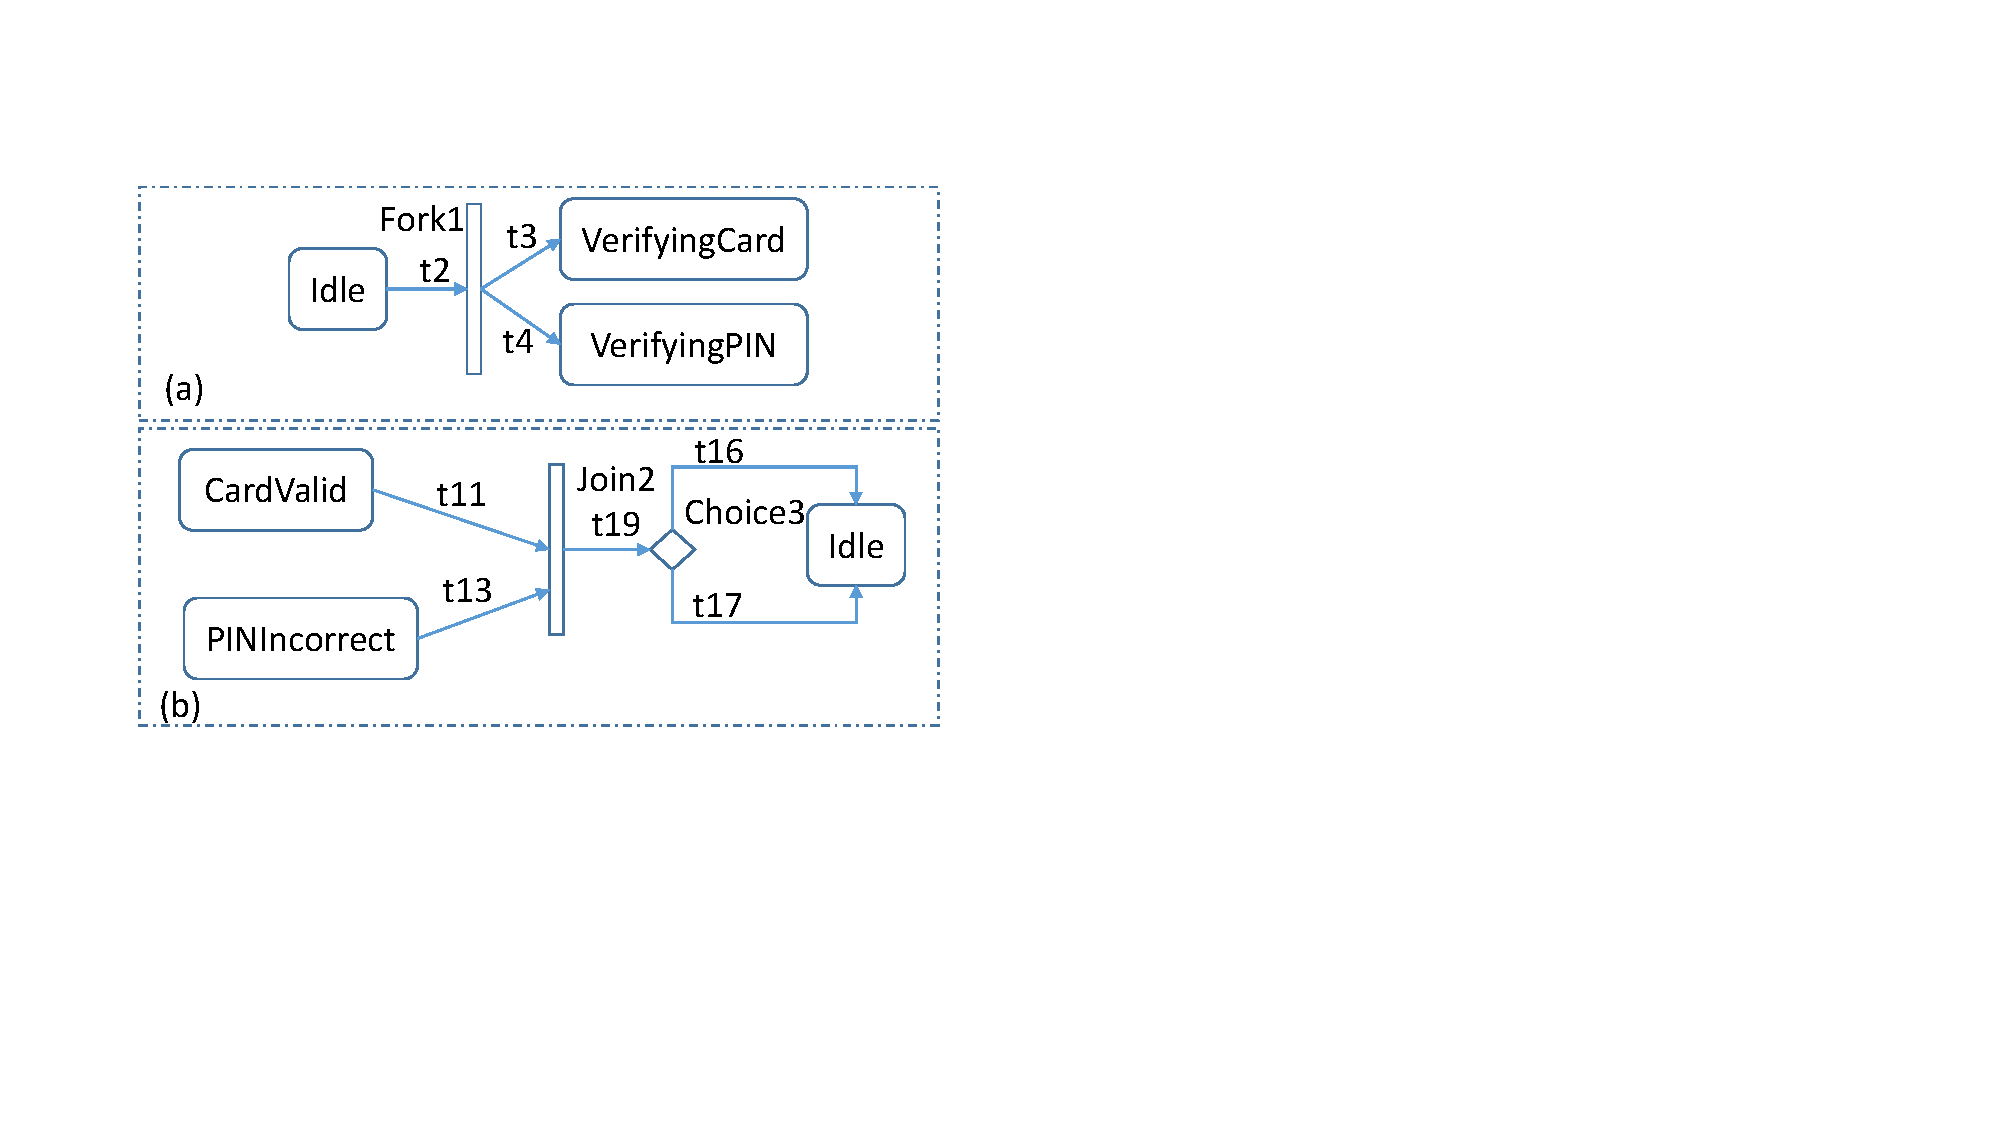
\includegraphics[clip, trim=2.0cm 6cm 17.5cm 3cm, width=\columnwidth]{figures/transitionGraph.pdf}
	\caption{Transition graphs} 
	\label{fig:transitionGraph}
\end{figure}


\begin{definition} A compound transition $t_{cp}$ is a virtual path which starts from one or multiple UML state and ends on one or multiple UML state. A compound transition is specified by a triple \{srcs($t_{cp}$), trc($t_{cp}$), tgts($t_{cp}$)\}, in which source part srcs($t_{cp}$) consists of one or multiple states, transition part trc($t_{cp}$) consists of multiple transitions, and target part tgts($t_{cp}$) consists of one or multiple states. 
\end{definition}


Given a state, Algorithm \ref{alg:cptransition} presents how to calculate transition graphs whose source $t_{cp}$ whose source part contains only a state $s$. 

\begin{algorithm}[]
	\caption{Transition graphs calculation
		\label{alg:cptransition}}
	\begin{algorithmic}[1]
		\Require{A state $s$ of a state machine}
		\Ensure{A set of transition graphs $\mathcal{GT}$}
		\Procedure{calculateTransGraphs}{$s$}
		\Let{$\mathcal{GT}$}{$\emptyset$} 
		\For {$out \in T_{outs}(s)$}
			\If {$tgt(out)$ is not a state}
				\Let{$\tau$}{($\mathcal{S}$, $\mathcal{L}$, $\mathcal{P}$, $\mathcal{T}$) $=\{\emptyset,\emptyset, \emptyset, \emptyset\}$}
				\Let{$\mathcal{P}$}{$\mathcal{P} \cup {tgt(out)}$}
				\Let{$\mathcal{S}$}{$\mathcal{S} \cup \{s\}$}
				\Let{$\mathcal{T}$}{$\mathcal{T} \cup {out}$}
				\If {$tgt(out).kind = join$}
					\Let{$ins$}{\\$\{i \in T_{ins}(tgt(out))| ctner(src(i)) = ctner(s)\}$}
					\Let{$\mathcal{S}$}{$\mathcal{S} \cup \{src(i)|i \in ins\}$}
					\Let{$\mathcal{T}$}{$\mathcal{T} \cup ins$}
				\EndIf
				\Let{$nexts$}{$FINDTRANS(tgt(out))$}
				\Let{$\mathcal{T}$}{$\mathcal{T} \cup nexts$}
				\Let{H}{\\$\{tgt(t)|t \in nexts \wedge tgt(t).kind = history\}$}
				\Let{$\mathcal{P}$}{$\mathcal{P} \cup \{src(t)|t \in nexts\} \cup H$}
				\Let{$\mathcal{L}$}{$\mathcal{L} \cup \{tgt(t)|t \in nexts \wedge tgt(t)$ is state $\}$}
								
				\Let{$\mathcal{GT}$}{$\mathcal{GT} \cup \{\tau\}$} 
			\EndIf
		\EndFor
		\EndProcedure
		
		\Require{A vertex $v$}
		\Ensure{Transition paths starting from $v$ and ending on a state}
		\Procedure{FindTrans}{$v$}
		\Let{$nextTrans$}{$T_{outs}(v)$}
		\For {$out \in T_{outs}(v)$}
			\If {$tgt(out)$ is not a state}
				\Let {$nextTrans$}{\\$nextTrans \cup FINDTRANS(tgt(out))$}
			\EndIf
		\EndFor	 			 	
		\Return {$nextTrans$} 
		\EndProcedure	
	\end{algorithmic}
\end{algorithm}

For example, applying this algorithm to all states of the state machine example in \ref{fig:example}, we can calculate other transition graphs which are:
\begin{IEEEeqnarray*}{lCr}
	\tau_{3} &=& (\mathcal{S}_3, \mathcal{L}_3, \mathcal{P}_3, \mathcal{T}_3) = (\{VerifyingCard\}, \{Idle, \\ 
	&& {} CardValid\}, \{Choice1\}, \{t5, t6, t7\}),
\end{IEEEeqnarray*}
\begin{IEEEeqnarray*}{lCr}	
	\tau_{4} &=& (\{VerifyingPIN\}, \{PINIncorrect, \\
	&& {} PINCorrect\}, \{Choice2\}, \{t8, t9, t10\}),
\end{IEEEeqnarray*} 
and
\begin{IEEEeqnarray*}{lCr}	
	\tau_{5} &=& (\{CardValid, PINCorrect\}, \{DispenseMoney\}, \\ 
	&& {} \{Join2\}, \{t12, t14, t15\}).
\end{IEEEeqnarray*} 

\end{comment}

\begin{comment}
\begin{definition} A transition graph $\tau$ is an acyclic directed graph ($\mathcal{T}_r$, $\mathcal{P}$, $\mathcal{T}$) where $\mathcal{P}$ is a set of vertexes, and $\mathcal{T}_{r}$ and $\mathcal{T}$ are sets of transitions. $\mathcal{T}_{r}$ is called the set of root transitions of the graph. Following conditions are satisfied:
	\begin{itemize}
		\item $\forall t \in \mathcal{T}_r, src(t)$ is a state.
		
		\item $\forall p \in \mathcal{P}, p.kind \notin \{state, comp, conc\}$.	
		
		\item $\forall t \in \mathcal{T}, src(t)$ is a pseudo state.
	\end{itemize}	
\end{definition}

A traversal from the root transitions of a transition graph to a stable state configuration is a compound transition. A state machine can contain multiple transition graphs. Fig. \ref{fig:transitionGraph} (a) and (b) show two transition graphs $\tau_{1}$ and $\tau_{2}$ of the ATM state machine, respectively, in which 
\begin{IEEEeqnarray*}{lCr}
	\tau_{1} &=& (\mathcal{T}_r, \mathcal{P}, \mathcal{T}) = (\{t2\}, \{Fork1\}, \{t3, t4\} )
\end{IEEEeqnarray*}
and
\begin{IEEEeqnarray*}{lCr}	
	\tau_{2} &=& (\{t11, t13\}, \{Join2, Choice3\}, \{t19, t16, t17\}).
\end{IEEEeqnarray*}



\begin{figure}
	\centering
	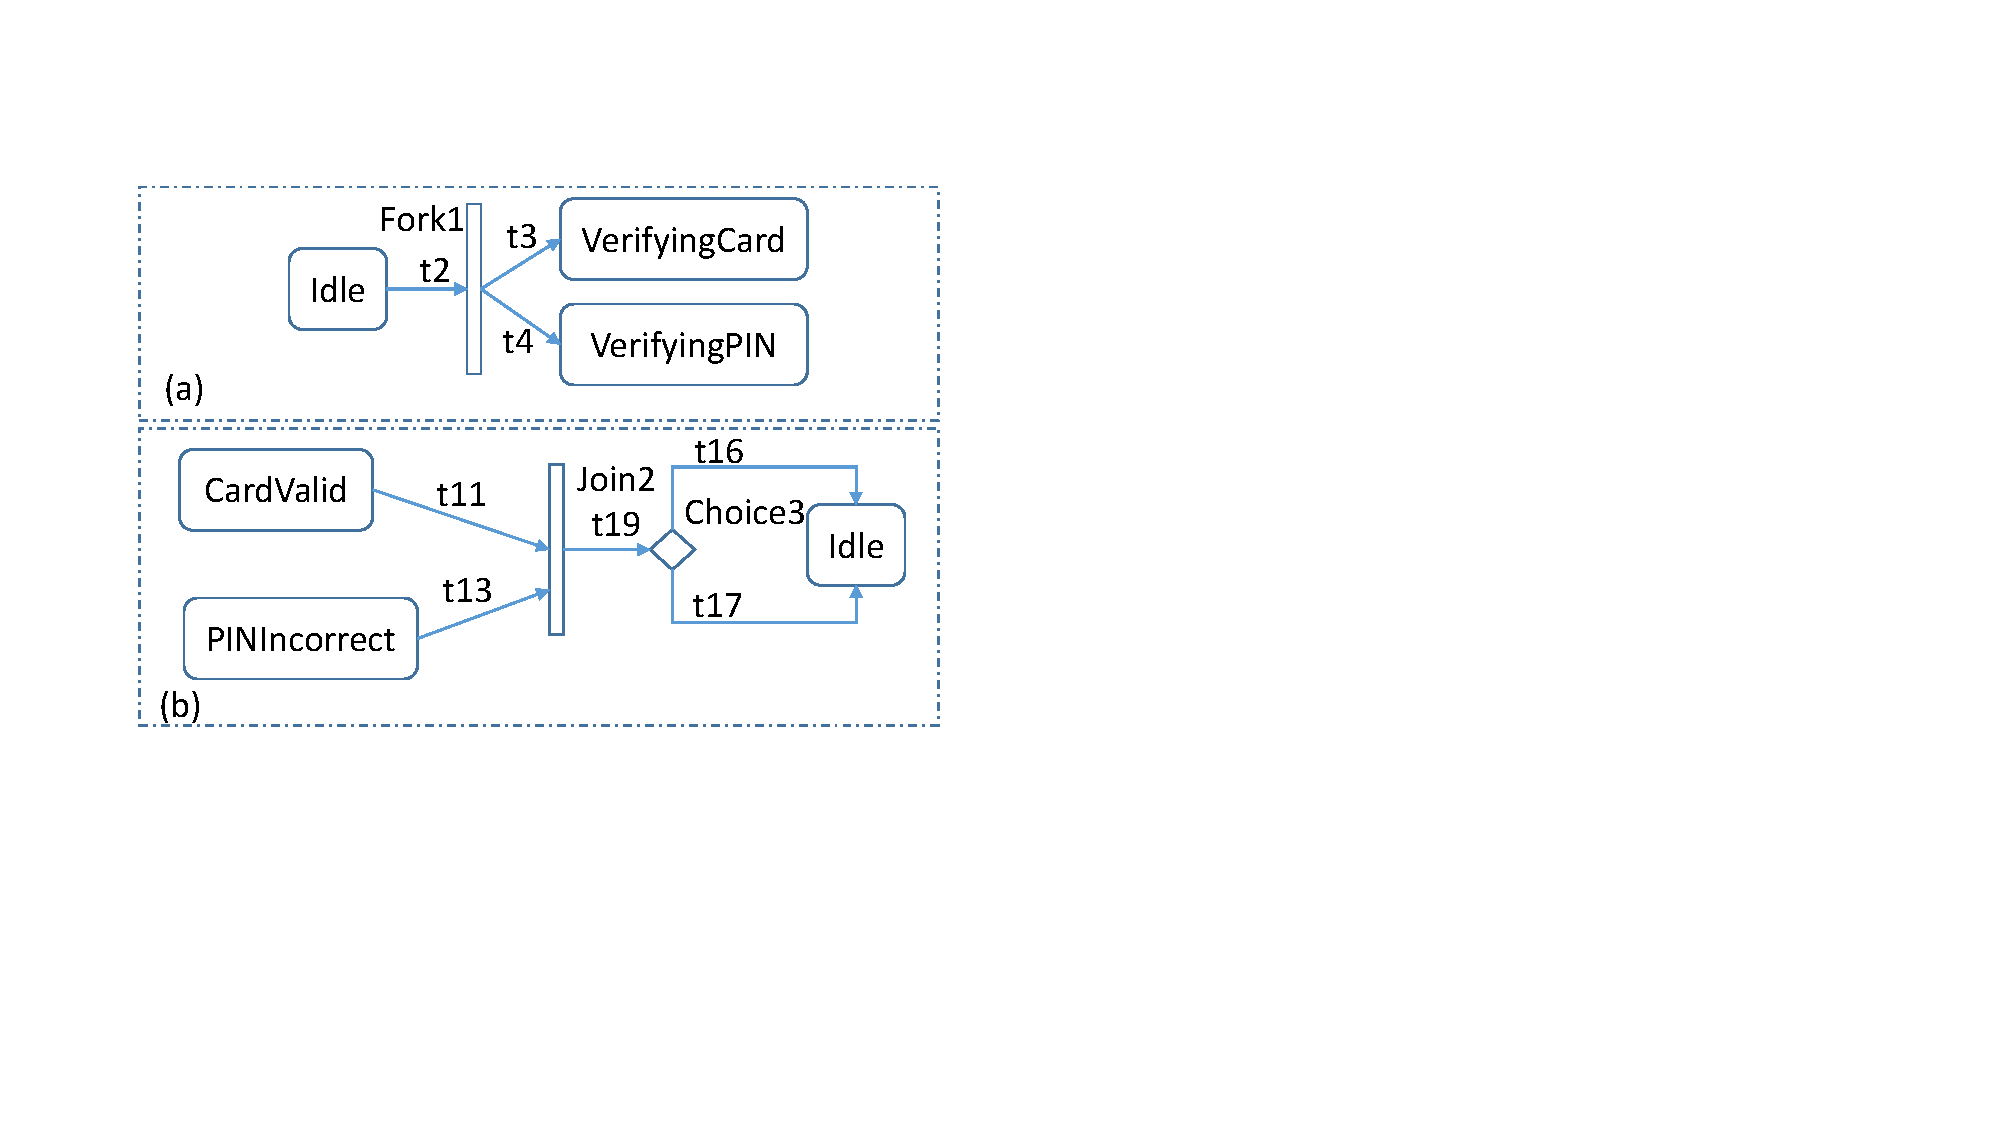
\includegraphics[clip, trim=2.0cm 6cm 17.5cm 3cm, width=\columnwidth]{figures/transitionGraph.pdf}
	\caption{Transition graphs} 
	\label{fig:transitionGraph}
\end{figure}



Given a state, Algorithm \ref{alg:cptransition} presents how to calculate transition graph set whose root transitions outgo from $s$. 

\begin{algorithm}[]
	\caption{Transition graphs calculation
		\label{alg:cptransition}}
	\begin{algorithmic}[1]
		\Require{A state $s$ of a state machine}
		\Ensure{A set of transition graphs $\mathcal{GT}$}
		\Procedure{calculateTransGraphs}{$s$}
		\Let{$\mathcal{GT}$}{$\emptyset$} 
		\For {$out \in T_{outs}(s)$}
			\If {$tgt(out)$ is not a state}
				\Let{$\tau$}{($\mathcal{T}_r$, $\mathcal{P}$, $\mathcal{T}$) $=\{\emptyset,\emptyset, \emptyset\}$}
				\Let{$\mathcal{P}$}{$\mathcal{P} \cup {tgt(out)}$}
				\Let{$\mathcal{T}_r$}{$\mathcal{T}_r \cup {out}$}
			\If {$tgt(out).kind = join$} 
				\Let{$\mathcal{T}_r$}{$\mathcal{T}_r \cup T_{ins}(tgt(out))$}
			\EndIf
				\Let{$nexts$}{$FINDTRS(tgt(out))$}
				\Let{$\mathcal{T}$}{$\mathcal{T} \cup nexts$}
			
				\Let{$\mathcal{GT}$}{$\mathcal{GT} \cup \{\tau\}$} 
			\EndIf
		\EndFor
		\EndProcedure
		
		\Require{A vertex $v$}
		\Ensure{Transition paths starting from $v$ to atomic  states}
		\Procedure{FINDTRS}{$v$}
		\Let{$outs$}{$T_{outs}(v)$}
		\For {$out \in T_{outs}(v)$}
			\If {$tgt(out)$ is not a state}
				\Let {$outs$}{\\$outs \cup FINDTRS(tgt(out))$}
			\ElsIf $tgt(out).kind \in {comp, conc}$
				\For {$sub \in subvertexes(tgt(out)), sub.kind=initial$}
					\Let {$outs$}{$outs \cup FINDTRS(sub)$}
				\EndFor
			\EndIf 
		\EndFor	 			 	
		\Return {$outs$} 
		\EndProcedure	
	\end{algorithmic}
\end{algorithm}

For example, applying this algorithm to all states of the state machine example in \ref{fig:example}, we can calculate other transition graphs which are:
\begin{IEEEeqnarray*}{lCr}
	\tau_{3} &=& (\mathcal{S}_3, \mathcal{L}_3, \mathcal{P}_3, \mathcal{T}_3) = (\{VerifyingCard\}, \{Idle, \\ 
	&& {} CardValid\}, \{Choice1\}, \{t5, t6, t7\}),
\end{IEEEeqnarray*}
\begin{IEEEeqnarray*}{lCr}	
	\tau_{4} &=& (\{VerifyingPIN\}, \{PINIncorrect, \\
	&& {} PINCorrect\}, \{Choice2\}, \{t8, t9, t10\}),
\end{IEEEeqnarray*} 
and
\begin{IEEEeqnarray*}{lCr}	
	\tau_{5} &=& (\{CardValid, PINCorrect\}, \{DispenseMoney\}, \\ 
	&& {} \{Join2\}, \{t12, t14, t15\}).
\end{IEEEeqnarray*} 

\end{comment}
\begin{definition} Current active configuration $Cfg$ of a UML state machine sm is a set of candidate UML states which are able to process an incoming event. 
\end{definition}







\section{experiments}
\lipsum
		



\section{Conclusion}
\label{sec:conclusion}
%\lipsum[1]


\bibliographystyle{plain}
\bibliography{references}


\end{document}
